\newcommand*\cols{2}
\newcommand*\rows{3}
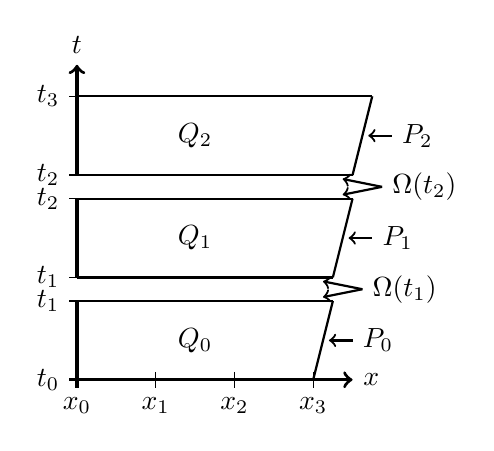
\begin{tikzpicture}[
    scale=1,
    axis/.style={very thick, ->},
    important line/.style={thick},
    newEdge/.style={thick, ->, >=circle},
    every node/.style={color=black}
    ]
    %x-axis
    \draw[axis] (-0.1,0)  -- (3.5,0) node(xline)[right]{$x$};
    \foreach \x in {0,1,2,3}
    \draw (\x cm,0.1) -- (\x cm,-0.1) node[anchor=north] {$x_{\x}$};
    % t-axis
    \draw[very thick] (0,-0.1) -- (0,1);
       \draw[very thick] (0,1.3) -- (0,2.3);
    \draw[axis] (0,2.6) -- (0,4) node(yline)[above]{$t$};
    \draw (0.1,0cm) -- (-0.1, 0cm) node[anchor=east] {$t_{0}$};
    \draw (0.1,1cm) -- (-0.1, 1cm) node[anchor=east] {$t_{1}$};
    \draw (0.1,1.3cm) -- (-0.1, 1.3cm) node[anchor=east] {$t_{1}$};
    \draw (0.1,2.3cm) -- (-0.1, 2.3cm) node[anchor=east] {$t_{2}$};
        \draw (0.1,2.6cm) -- (-0.1, 2.6cm) node[anchor=east] {$t_{2}$};
            \draw (0.1,3.6cm) -- (-0.1, 3.6cm) node[anchor=east] {$t_{3}$};
    % Lines
    \foreach \i / \row in {0/0, 1/1.3, 2/2.6} {
     		\foreach \col in {0, 1, ...,\cols} {
   				 \draw[important line] (\col,\row) coordinate (A)  -- (\col+1+0.25*\i,\row) coordinate (B);
   				 \draw[important line] (\col,\row+1) coordinate (A)  -- (\col+1+0.25*\i+0.25,\row+1) coordinate (B);
				 %\draw[important line, color=green] (\col,\row) coordinate (A)  -- (\col,\row+1) coordinate (B);
   				 %\fill (A) circle (2pt);
   				 %\fill (B) circle (4pt);

   				 %\fill (A) circle (2pt);
   				 %\fill (B) circle (3pt);
				%\draw[important line, color=magenta] (\col+0.25*\row,\row) coordinate (A)  -- (\col+1+0.25*\row+0.25,\row+1) coordinate (B);
   		 }		  
   	    \draw[important line] (\cols+1+0.25*\i,\row) coordinate (A)  -- (\cols+1+0.25*\i+0.25,\row+1) coordinate (B);   		  \node (Q) at (1.5,0.5+\row) {$Q_{\i}$};		  
        \draw[thick,<-] (3.2+0.25*\i,0.5+\row) -- (3.5+0.25*\i, 0.5+\row) node[anchor=west] {$P_{\i}$};
    }
    \draw[thick,<-] (3.0+0.25*0.5,1.25cm) -- (3.5+0.25*0.5, 1.15) node[anchor=west] {$\Omega(t_1)$};
    \draw[thick,<-] (3.0+0.25*0.5,1.05cm) -- (3.5+0.25*0.5, 1.15);
    \draw[thick,<-] (3.0+0.25*1.5,2.35cm) -- (3.5+0.25*1.5, 2.45) node[anchor=west] {$\Omega(t_2)$};
    \draw[thick,<-] (3.0+0.25*1.5,2.55cm) -- (3.5+0.25*1.5, 2.45);
\end{tikzpicture}
